\documentclass{article} % For LaTeX2e
\usepackage[utf8x]{inputenc}
\usepackage[T1]{fontenc}
\usepackage{nips11submit_e,times}
\usepackage{natbib}
\usepackage{amsmath}
\usepackage{graphicx}
%\documentstyle[nips10submit_09,times,art10]{article} % For LaTeX 2.09


\title{A Common GPU N dimensions array}


\author{
Frédéric Bastien\thanks{ Use footnote for providing further information
about author (webpage, alternative address)---\emph{not} for acknowledging
funding agencies.} \\
D\'epartement d'Informatique et de Recherche Op\'erationelle\\
Universit\'e de Montr\'eal\\
Montr\'eal, Canada \\
\texttt{nouiz@nouiz.org} \\
\And
Arnaud Bergeron \\
Lisa Laboratory \\
Universit\'e de Montr\'eal \\
\texttt{bergearn@iro.umontreal.ca} \\
\AND
Yoshua Bengio \\
D\'epartement d'Informatique et de Recherche Op\'erationelle \\
Universit\'e de Montr\'eal \\
\texttt{bengioy@iro.umontreal.ca} \\
}

% The \author macro works with any number of authors. There are two commands
% used to separate the names and addresses of multiple authors: \And and \AND.
%
% Using \And between authors leaves it to \LaTeX{} to determine where to break
% the lines. Using \AND forces a linebreak at that point. So, if \LaTeX{}
% puts 3 of 4 authors names on the first line, and the last on the second
% line, try using \AND instead of \And before the third author name.

\newcommand{\fix}{\marginpar{FIX}}
\newcommand{\new}{\marginpar{NEW}}

\nipsfinalcopy % Uncomment for camera-ready version

\begin{document}


\maketitle

\begin{abstract}
Currently there is multiple array/matrix/n-dimensional array object
that exist on the gpu.  This hinder sharing gpu code and cause
duplicate development work. This paper present a proposition and a
first version~\citep{GpuNdArray} for a common gpu n-dimensional
array(tensor) on the GPU. It will work on CUDA and OpenCL. It will be
usable in python, C++ and possibly others languages.
\end{abstract}

\section{Introduction}
Currently there is at least 4 differents gpu array in python:
CudaNdarray(Theano), GPUArray(pycuda) and CUDAMatrix(cudamat),
GPUArray(pyopencl). There is also other implementation like Trust in
C++.  The problem is that they are not compatible with each
others. All of them have the caracteristic of being a subest of a
tensor(n-dimensional array) that support strides like what
Numpy~\citep{numpy-2007} provides on the CPU.

Strides are a way to specify the number of element to skip when going
to the next element in a gived dimensions.  As an example, this allow
to make a view that represent only odd, even, every third row, ... on
a matrix. This avoid coping data and lower the memory usage and memory
access. More generally this allow to make a view on existing tensor
memory space while the view see only some part of it. A part can be
specified for each dimensions and can be a range of elements with a
step different then 1 between each consecutive elements in the
view. We represent them as slice with a start(include) index, an
end(excluded) index and a step.


We think that one of the reason why there is so many differents bases
objects is that on the gpu, implementing a general tensor with strides
make coding for GPU even harder. This can be easily bypassed by using
function to check/convert some condition on the memory layout. For
example, if a developer want to only consider inputs in C or Fortran
order for one function, he could just call a function on his inputs to
convert the input into its supported inputs layout.

A second reason why people didn't implemented all those feature is
that having more dimensions and having strides strides take more
computation for indexing. This can lead the slower code. We will take
as example the addition of 2 tensors of 10 dimensions. In serial code,
having more dimensions just add more imbricated loop. If the inner
loop is big enought, having more loopo on top probably won't make big
different. In parallel code, this is not trivial to have indexing
computation not significant for big number of dimensions. CUDA can
provide only up to 5 implicit loop. So all extra dimensions request
additional indexing computation. Also, if the size of those dimensions
are not suited to the GPU, this can lead to lower performance.

There is optimization possible for computating the indexing like
collapsing some dimensions on the cpu and invisibly using a kernel
that support less dimensions. The trick come from knowing witch
dimensions you can collapse for witch function and inputs. This is
implemented for elemwise operation as discussed in the ``Current
implementation'' section.

We think that if we provide such optimized function for elemwise and
reduction operation, we will cover enough case where conversion from
one memory layout to another can be combiend with computation. This
can still impact the performance due to coalescing constrain, but we
don't expect that to be significant most of the time.


The lack of a common GPU tensor create many problems. Here is a few:
\begin{itemize}
  \item Duplicate work
  \item Harder to port/reuse code
  \item Harder to find/distribute code
  \item Divides development work
\end{itemize}

All those problem are agravated by the fact that GPU code is
harder/slower to do correctly and fast than serial CPU code.

\subsection{Pitfall to Avoid}
\begin{itemize}
\item Start alone
  \begin{itemize}
  \item We need different people/groups to ``adopt'' the new GpuNdArray
  \end{itemize}
\item Too simple(ex: just a 1d array) - other projects won't adopt as it won't fit there need.
\item Too general - other projects will implement ``light'' version... and not adopt
  \begin{itemize}
  \item Having an easy way to convert/check conditions could alleviate this.
  \end{itemize}
\end{itemize}

\subsection{Goal/Strategy}
The goal is to have a common GPU object that will be used by every body. We think that the best strategy is:

\begin{itemize}
\item Make a n dimensionals array on the gpu that support strides
\item Make the python interface similar to numpy.ndarray
  \begin{itemize}
  \item Easier to attract other peole from python community
  \end{itemize}
\item Have the base object in C to allow collaboration with more project.
  \begin{itemize}
  \item  want people from C, C++, ruby, R, ... all use the same base Gpu ndarray.
  \end{itemize}
\item Be compatible with CUDA and OpenCL
\end{itemize}


We think that for a common GPU object, we need an n dimensionals
array. This is motivated that forcing user to use an object that
support only 1 or 2 dimensions add complexity to the user when he need
to deal with algorithms that have natively more then 2 dimensions. We
don't think that this complexity should be deal by each users for each
such problems. Having a base object that support n-dimensions, remove
this coding complexity from the user point of view.

From the developer point of view, sometimes it is worth to support
strided tensor as inputs. But this is not the case. We don't think
that asking the developers that choose to don't support n-dimensionals
inputs to call a function to assert/convert the inputs memory layout
is something too complicated or time consuming. Especially when those
functions are provided and compared again reimplementing its own objects.

Many times, the inputs layout choosed by the developer of a function
will lead to better memory access pattern then a random memory
layout. So this is not trivial to say that generalizing the
implementation to support general memory layout will lead to
significant performance gain. If someone else want to use this
implementation without having this memory layout conversion, he could
genearalize it himself. But having a working implementaiton is really
useful to get started and help in the frequent case where this is not a
bottleneck in your code.



\section{Existing Implementation}
\subsection{Theano(CudaNdarray)}
Theano is the more high level system that provide an implementation of a subset of a gpu tensor. From its web site Theano~\citep{bergstra+al:2010-scipy} is:
``a Python library that allows you to define, optimize, and evaluate mathematical expressions involving multi-dimensional arrays efficiently''. The web site also high that it have a ``tight integration with numpy'', ``transparent use of GPU'', ``efficient symbolic differentiation'', ``speed and stability optimization'', ``dynamic C code generation'' and ``extensive unit-testing and self verification''.

It implement a gpu tensor with strides, but support only float32 and CUDA. Also, the strides informations are stored differently then numpy. Theano store in with the number of element to skip to access the next element. Numpy store the number of bytes.

We prefer to use the number of bytes as restricting ourself to number of element restrict us to tensor with homogenous data. We can't have the element be a struct of (float32,uint8), then take a view of only the float32 part. We currently don't support this, but we don't want to prevent us or someone else to add this in the futur.

\subsection{PyCUDA/PyOpenCL(GPUArray)}
PyCUDA~\citep{kloeckner_pycuda_2009} and PyOpenCL~\citep{kloeckner_pycuda_2009} are python wrapper around CUDA and PyOpenCL respectively. In addition to wrapping their respective library, it do automatic Object clean up, it add a gpu array object and some abstraction for compilation. It also automatically transfort errors to python exceptions.

There gpu array object are limited to contiguous memory region. It add a shape properties to allow using this contiguous memory region as n-dimensional array, but it don't work with strides. Both projects can be used together in the same python script. Also, it support many dtypes.

\subsection{CUDAMat}
The CUDAMat~\citep{cudamat-TR2009} web site describe well itself: ``The aim of the cudamat project is to make it easy to perform basic matrix calculations on CUDA-enabled GPUs from Python. cudamat provides a Python matrix class that performs calculations on a GPU.''

So we clearly see that it support only CUDA and matrix. If we look deeper we see that it don't support strides and support only float32 datatype.

\subsection{Gnumpy}
Gnumpy~\citep{gnumpy-TR2010} is on top of cudamat. It add many functionality on the gpu. It allow to work with n-dimentional array when they are contiguous in memory. So no support for strides. It also add support for bollean type by using 1.0 and 0.0 in float32 to represent a boolean value.

\subsection{Trust}
Trust~\citep{Thrust} is a C++ template library. It provide a vector object for cuda. It support all dtype, but no strides.

\subsection{Summary}
We see clearly that none of those implementation offer what we want for a common gpu tensor. As Theano implementation support strides and that it is easier to add multiple dtype then to add strides support, we used many of its code as a base of our implementation. Theano also implemented some optimization to lower the performance loss of having more

\section{Current implementation}

Multiple backend:
Current behavior not wanted
    * No CPU code generated from the python interface(for PyOpenCL and PyCUDA) Gpu code are ok.

\subsection{Functionality}

The current code can allocate arrays, transfer data to and from the CPU, create view of that data and run elementwise kernels on that data.  In order to support multiple APIs we have created a list of utility functions that are to be implemented for each API and the rest of the code is shared.

The language independent parts take care of indexing, making views, and provide an API that is very similar to numpy.  This is the part that supports any (valid) combination of dimensions and strides.  \emph{(mabye) Most importantly, the element-wise kernels and dimension collapsing optimizations are device-independent and can be reused between APIs.}

We are still missing some items before we reach full numpy compatibility, most importantly setting a part of the array via assignation and reshaping.

fct implemented language dependent
cuda
malloc/free
memcopy
memset
from cpu to gpu
from gpu to cpu

gpu agnos:
sub tensor
deepcopy
view
zeros
empty

probably gpu agnos, not sure:
elemwise
elemwise dimensions collapsing


todo:
assignation
reshape
n dimensional tranpose
dot22,gemm
reduce along all dimensions, along one axis or a list of dimensions
reduce dimensions collapsing

\subsection{Elemwise dimensions collapsing}
TODO

\section{Benchmarks}

In order to measure the overhead of multiple dimensions and strides in comparison to existing implementations, we compared some elementwise kernels generated with PyCUDA to some generated using our algorithm (including dimension collapsing and strides data).  The timings shown below do not include any transfer time or allocation of output array.  They were made on a GTX 580.

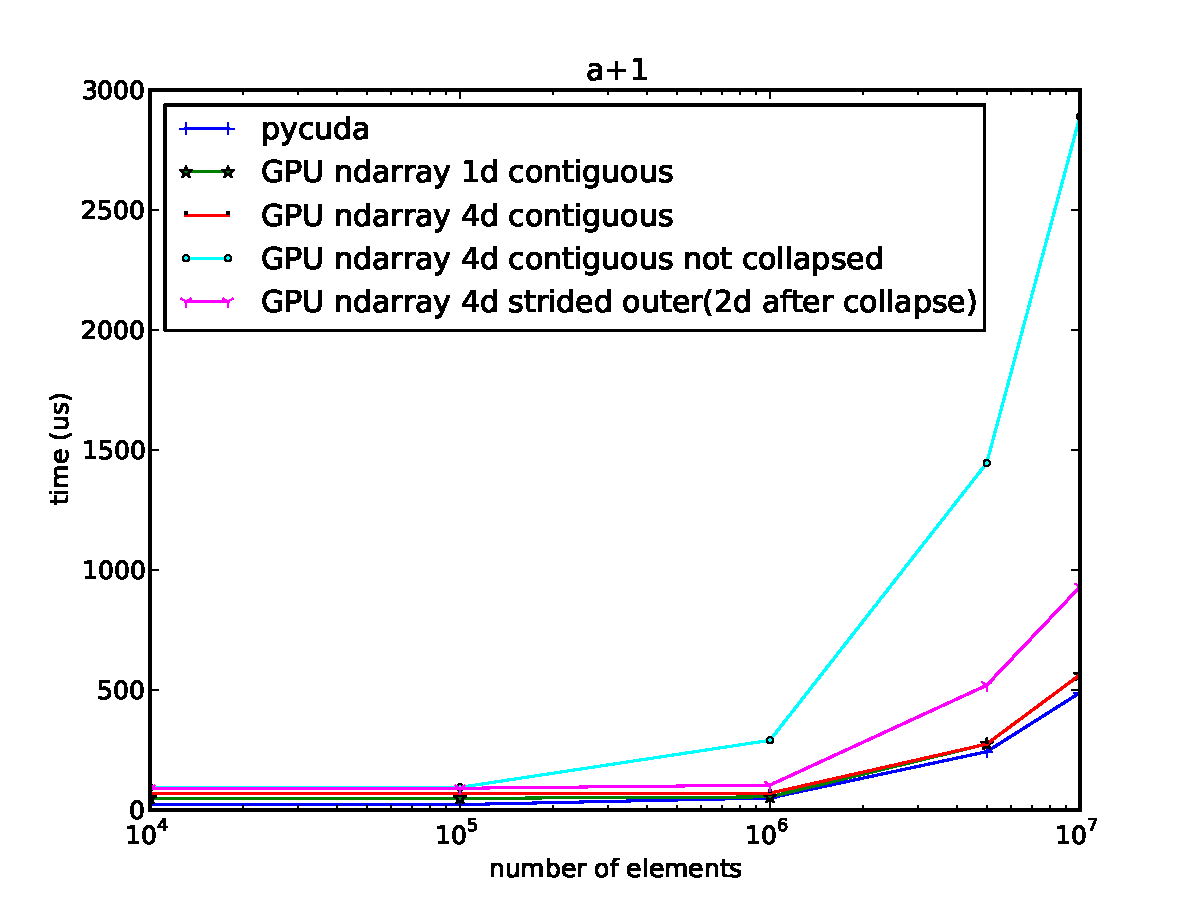
\includegraphics[width=0.5\textwidth]{ap1_no_alloc}
\includegraphics[width=0.5\textwidth]{apb_no_alloc}
\includegraphics[width=0.5\textwidth]{2ap3b_no_alloc}
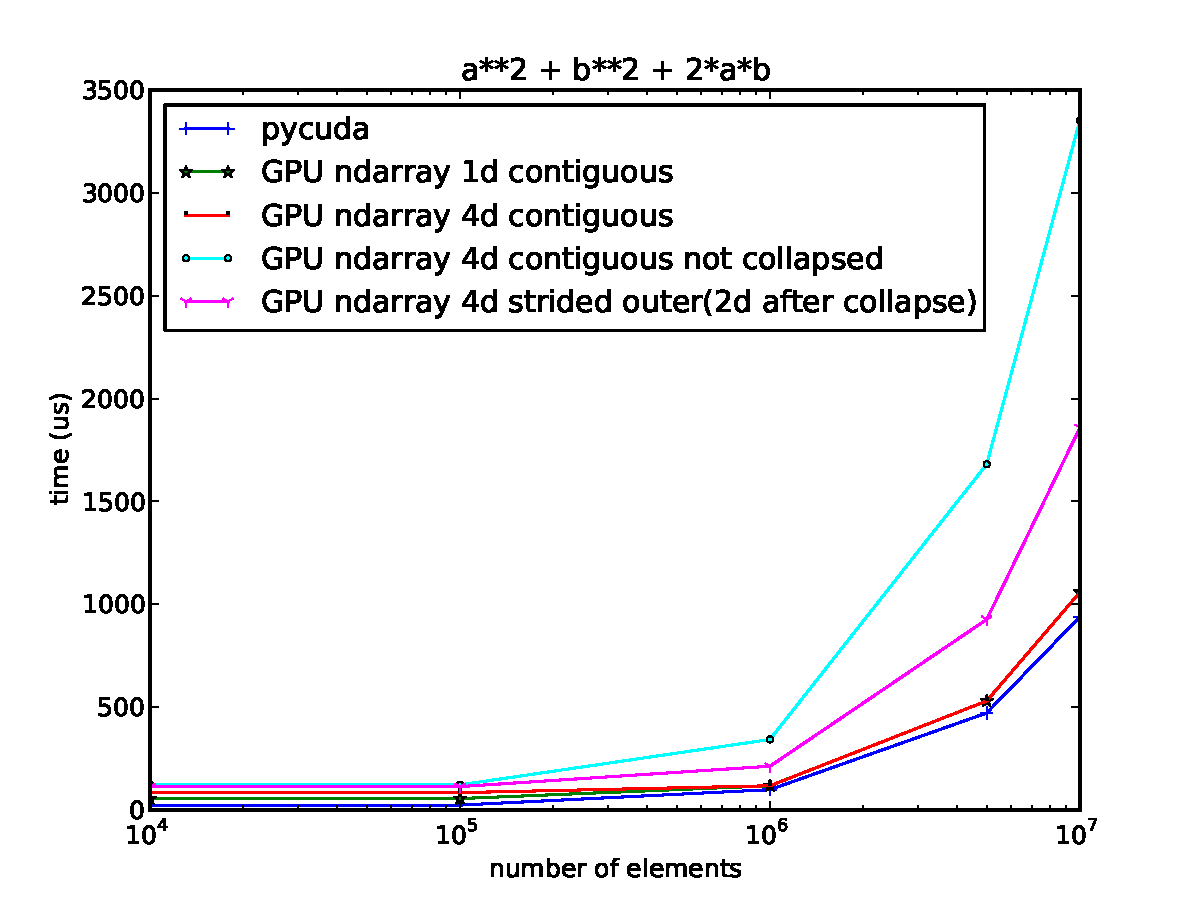
\includegraphics[width=0.5\textwidth]{a2pb2p2ab_no_alloc}

We can conclude from these benchmarks that we have a bigger base cost that PyCUDA.  Although it is interesting to note that the strides code does not add any significant overhead to the computations.

\section{Future Plans}
\section{Conclusion}

%\subsection{Margins in LaTeX}
% 
%Most of the margin problems come from figures positioned by hand using
%\verb+\special+ or other commands. We suggest using the command
%\verb+\includegraphics+
%from the graphicx package. Always specify the figure width as a multiple of
%the line width as in the example below using .eps graphics
%\begin{verbatim}
%   \usepackage[dvips]{graphicx} ... 
%   \includegraphics[width=0.8\linewidth]{myfile.eps} 
%\end{verbatim}
%or % Apr 2009 addition
%\begin{verbatim}
%   \usepackage[pdftex]{graphicx} ... 
%   \includegraphics[width=0.8\linewidth]{myfile.pdf} 
%\end{verbatim}
%for .pdf graphics. 
%See section 4.4 in the graphics bundle documentation (http://www.ctan.org/tex-archive/macros/latex/required/graphics/grfguide.ps) 
% 
%A number of width problems arise when LaTeX cannot properly hyphenate a
%line. Please give LaTeX hyphenation hints using the \verb+\-+ command.


\subsubsection*{Acknowledgments}

We want to thanks James Bergstra. We used some of his code as the first version of some functionality currently implemented. I would also like to acklowledge Compute Canada, RQCHP, NSERC, and Canada Research Chairs for providing fonds or access to compute ressource.


\bibliography{strings,strings-shorter,ml,aigaion-shorter}
\bibliographystyle{plain}

\end{document}
